\begin{comment}
\textbf{Asignatura: Pensamiento Económico e instituciones}\\
\textbf{Máster en Economía}\\
\textbf{Universidad de Vigo, Santiago de Compostela y La Coruña}\\
\end{comment}
\begin{center}
\textbf{\Large Crecimiento y libertad económica: Un análisis cuantitativo}\\
\vspace{0.5cm}
\textbf{Por FODE (Christian Limbert Paredes Aguilera)}\\
\end{center}
\vspace{1cm}

    \section*{Introducción}
    Este trabajo tiene el propósito de analizar cuantitativamente la relación que existe entre el crecimiento económico y la libertad económica, por lo que recogeremos y organizaremos datos del instituto Fraser, del Penn World Table, de programad de desarrollo de las naciones unidas, de la universidad de Yale y del Banco Mundial. Dicho análisis se realizará para 112 países con el método de regresión de convergencia mediante  el entorno y lenguaje de programación R.\\
    El objetivo principal del modelo es, por un lado, ver si se cumple la convergencia del modelo de Solow donde los países que partían de un menor PIB pc tenían un crecimiento más rápido que los que partían de un PIB pc mayor y, por otro lado, analizar las variables de las que se componen la libertad económica y ver como se correlacionan con el crecimiento económico.

    \section*{Análisis descriptivo del índice de libertad económica y sus componentes}

    Libertad económica significa el grado en que existe una economía de mercado, donde los componentes centrales son el intercambio voluntario, la libre competencia y la protección de las personas y la propiedad (Gwartney y Lawson 2002, 5). El objetivo es caracterizar la estructura institucional y las partes centrales de la política económica. La libertad económica puede constituir un factor explicativo del crecimiento y de la distribución del ingreso. En el análisis econométrico, la libertad económica es, por tanto, una variable independiente. Sin embargo, la libertad económica también puede verse afectada por otras variables y, por lo tanto, constituir una variable dependiente, posiblemente influenciada por factores como la libertad política, la riqueza o la democracia.\\

    El intento más ambicioso de cuantificar la libertad económica es el Índice de Libertad Económica (EFI) que se informa anualmente en Economic Freedom of the World (Gwartney y Lawson 2002). Desde 1996, se han publicado datos actualizados anualmente, y los datos ahora cubren los años 1970, 1975, 1980, 1985, 1990, 1995 y 2000. Estos datos han comenzado a usarse en investigaciones académicas, que ha contribuido a aumentar nuestro conocimiento sobre la importancia de la libertad económica.\\
    Otro índice de este tipo es publicado por la Heritage Foundation en cooperación con el Wall Street Journal (O'Driscoll, Holmes y O'Grady 2002).3 Este índice y el EFI son similares en sus implicaciones generales, pero debido a que se ha utilizado el EFI más extensamente en contextos académicos.

    \subsection*{El concepto de libertad económica}
    La libertad económica es un compuesto que intenta caracterizar el grado en que una economía es una economía de mercado, es decir, el grado en el que implica la posibilidad de celebrar contratos voluntarios dentro del marco de un estado de derecho estable y predecible que respeta los contratos. Y protege la propiedad privada, con un grado limitado de intervencionismo en forma de propiedad del gobierno, regulaciones e impuestos. 
    El EFI es un medio de medir el grado de libertad económica al incluir treinta y siete componentes divididos en cinco grupos en un índice para los años, 1990 (113 países), 1995 (123 países) y 2000 (123 países). Los cinco grupos son: 

    \begin{enumerate}

	\item[Área 1.] \textbf{Tamaño del gobierno}.- A medida que aumentan el gasto público, los impuestos y el tamaño de las empresas controladas por el gobierno, la toma de decisiones del gobierno sustituye a la elección individual y se reduce la libertad económica.

	\item[Área 2.] \textbf{Sistema legal y derechos de propiedad}.- La protección de las personas y su propiedad legítimamente adquirida es un elemento central tanto de la libertad económica como de la sociedad civil. De hecho, es la función más importante del gobierno.

	\item[Área 3.] \textbf{La inflación monetaria sólida}.- erosiona el valor de los salarios y ahorros ganados legítimamente. Por lo tanto, el dinero sólido es esencial para proteger los derechos de propiedad. Cuando la inflación no solo es alta sino también volátil, se vuelve difícil para las personas planificar el futuro y, por lo tanto, utilizar la libertad económica de manera eficaz.

	\item[Área 4.] \textbf{Libertad para comerciar internacionalmente}.- La libertad para intercambiar —en su sentido más amplio, comprar, vender, hacer contratos, etc., es esencial para la libertad económica, que se reduce cuando la libertad de intercambiar no incluye empresas e individuos de otras naciones.

	\item[Área 5.] \textbf{Regulación}.- Los gobiernos no solo usan una serie de herramientas para limitar el derecho a intercambiar internacionalmente, sino que también pueden imponer regulaciones onerosas que limitan el derecho a intercambiar, obtener crédito, contratar o trabajar para quien usted desee u operar libremente su negocio.

    \end{enumerate}

    Cada componente se mide de 0 (sin libertad económica) a 10 o 100 (plena libertad económica). El índice se calcula utilizando promedios aritméticos.\\

    \begin{center}
	Tabla 1: Libertad económica\\(2017)\\
	\begin{tabular}{r|c}
	    \hline
	    \textbf{País} & \textbf{Indice} \\
	    \hline
	    Hong Kong & 89.8 \\
	    Estonia & 79.1 \\
	    Israeil & 69.7 \\
	    Burkina Faso & 59.6 \\
	    Mozambique & 49.9 \\
	    Venezuela & 27.0 \\
	    \hline
	\end{tabular}\\
	\small{Fuente: propia}
    \end{center}
    \vspace{.5cm}

    La Tabla de arriba presenta los valores de EFI en 2017 para varios países, en sus distintas categorías. En números absolutos, un pequeño país asiático junto con Estonia ocupan los puestos de arria. Al fondo, se encuentra Venezuela; varias naciones africanas también ocupan puestos bajos, tal es caso de Burkina Faso o Mozambique.\\


    \begin{center}
	Tabla 2: Libertad económica para EEUU.\\
	(1970-2000)\\
	\begin{tabular}{cccccccc}
	    \hline
	    Año&Rank&EFI&Gobierno&Legal&Moneda&Comercio&Regulación\\
	    \hline
	    1970&11&7.0&4.0&8.3&9.6&7.0&5.9\\
	    1975&3&7.3&4.8&7.9&9.2&7.7&6.7\\
	    1980&4&7.5&5.2&8.3&9.2&8.0&6.8\\
	    1985&5&7.7&6.0&8.3&9.3&7.8&6.8\\
	    1990&3&7.9&6.8&8.3&9.6&7.8&6.8\\
	    1995&4&8.3&6.9&8.6&9.7&7.9&8.3\\
	    2000&3&8.5&7.6&9.2&9.7&8.0&8.2\\
	    \hline
	\end{tabular}\\
	\small{Fuente: Gwartney and Lawson 2002, 165}
    \end{center}

    En la tabla 2 se presentan datos más detallados para los Estados Unidos. Los puntajes de los Estados Unidos son altos en todos los ámbitos. Se han realizado mejoras en todas las áreas durante el período estudiado, especialmente con respecto al tamaño del gobierno. El índice permite a los investigadores realizar análisis estadísticos de la importancia de la libertad económica. Al examinar la construcción del índice, se encuentra que se basa en gran parte en datos publicados en fuentes secundarias, que por lo tanto pueden verificarse fácilmente. Además, es fácil asignar nuevos pesos a los componentes del índice si así se desea.\\

    \subsection*{La importancia de la libertad económica}
    En la medida en que las instituciones estimulen acciones que contribuyan a la producción de productos más valiosos, contribuirán al crecimiento económico. Las instituciones que garantizan la libertad económica plausiblemente tienen la capacidad de proporcionar el tipo de incentivos que mejoran el crecimiento, por varias razones: promueven un alto rendimiento de los esfuerzos productivos a través de impuestos bajos, un sistema legal independiente y la protección de la propiedad privada; permiten que el talento se asigne donde genera el valor más alto (como se argumenta en Murphy, Schleifer y Vishny 1991); fomentan una economía dinámica, organizada experimentalmente, en la que puede tener lugar una gran cantidad de ensayo y error comercial (Johansson 2001, cap. 2) y en la que se produce competencia entre diferentes actores porque las regulaciones y las empresas gubernamentales son pocas; facilitan la toma de decisiones predecibles y racionales a través de una tasa de inflación baja y estable; y promueven el flujo de comercio e inversión de capital hacia donde la satisfacción de preferencias y los rendimientos son más altos.\\

    No es difícil afirmar que es probable que la libertad económica tenga un efecto favorable en la prosperidad económica, por la sencilla razón de que los últimos cincuenta años de experiencia internacional confirman más o menos el hecho de que dondequiera que los gobiernos usaron más los mercados y adoptaron políticas más abiertas en el comercio exterior y la inversión, de hecho en más libertad económica de diferentes tipos, sus países han tendido a prosperar. Por el contrario, aquellos países que se volvieron hacia adentro y tenían regulaciones extensas de todo tipo sobre la toma de decisiones económicas internas en producción, inversión e innovación, son los países que realmente no lo han hecho demasiado bien.\\

    \begin{center}
	Figura 1: Libertad económica y crecimiento del PIB per cápita.\\
	1990-2000\\
	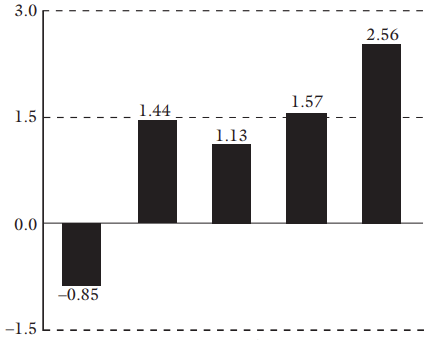
\includegraphics[scale=.5]{codigoFuente/tareas/pensamiento/img/1pensamiento.png}\\
	Quantiles EFI\\
	\small{Fuente: Gwartney and Lawson 2002,20}
    \end{center}

    Como muestra la figura, la quinta parte de los países que han tenido la libertad económica más alta han crecido considerablemente más rápido que otros países, mientras que la quinta parte de los países con la libertad económica más baja han tenido, de hecho, un crecimiento negativo. \\
    Gwartney, Lawson y Holcombe (1999), encuentran que el nivel de libertad económica al comienzo del período de crecimiento estudiado no contribuye significativamente explicar el crecimiento, pero que los cambios positivos en la libertad económica sí lo hacen. Por otro lado se encontró que el nivel inicial de libertad económica está positivamente relacionado con el crecimiento (Ali 1997; Easton y Walker 1997; Goldsmith 1997; Dawson 1998; Wu y Davis 1999; Hanson 2000; Heckelman y Stroup 2000;10Ali y Crain 2001 , 2002; Carlsson y Lundström 2002; Pitlik 2002; Scully 2002; Weede y Kämpf 2002). En varios de estos casos el efecto de nivel parece estadísticamente significativo solo si el cambio en la libertad económica también se incluye como variable.\\

    Algunas partes del EFI pueden promover el crecimiento más que otras. Carlsson y Lundström (2002) establecen que de los siete grupos EFI (en la versión publicada en 2000), cuatro se relacionan positiva y estadísticamente significativamente con el crecimiento (estructura económica y uso de mercados, libertad de uso de monedas alternativas, estructura legal y seguridad de propiedad y la libertad de intercambio en los mercados de capital), dos están negativamente y estadísticamente significativamente relacionados con el crecimiento (el tamaño del gobierno y el intercambio internacional/libertad para comerciar con extranjeros), y uno no está estadísticamente relacionado con el crecimiento (política monetaria y precios. Estabilidad). Lo más sorprendente de estos resultados, tanto desde una perspectiva teórica como en comparación con otros resultados empíricos, son las dos relaciones negativas detectadas. Implican que cuanto menor sea el tamaño del gobierno y mayor la libertad para comerciar con extranjeros, más lenta será la tasa de crecimiento. Una dificultad con las mediciones agregadas de este tipo es que ciertas empresas públicas pueden tener efectos de crecimiento positivos, mientras que otras tienen efectos negativos. 
    Otros estudios analizan el crecimiento o producto interno bruto (PIB) per cápita en función de la libertad económica o sus componentes. En general, los resultados son compatibles con los mencionados anteriormente, y aquí se presenta una selección de estos estudios.\\

    Los resultados más importantes se resumen en el cuadro 3. No se han informado resultados que muestren que la libertad económica obstaculiza el crecimiento o que está asociada con un PIB per cápita más bajo. Por el contrario, los resultados en general muestran que un aumento de la libertad económica ejerce una influencia positiva en el desarrollo de la riqueza económica.\\

    \begin{center}
	Tabla 3: El efecto de la libertad económica en el crecimiento y el PIB per capita
	\scalebox{0.8}{
	\begin{tabular}{lccc}
	    \hline
	    Estudios & Variable dependiente & Variable independiente & Efecto \\
	    \hline
	    Dawson 1998, forthcoming,&&&\\
		     Gwartney, Lawson, y&Crecimiento&Cambio en la EFI&Significativa\\
					Holcombe 1999, de Hann&&&positivo\\
					y Sturn 2000,2001;&&&\\
					Adkins, Moomaw, y&&&\\
					Savvides 2002; Pitlik 2002;&&&\\
								   Weede y Kampf 2002&&&\\
												  \hline
										     Gwartney, Lawson y &Crecimiento&Nivel de la EFI&No\\
										     Holcombe 1999; de Hann y&&&significativo\\
										     Sturm 2000, 2001;&&&\\
										     Heckelman y Stroup 2000;&&&\\
										     Adkins, Moomaw, y&&&\\
										     Savvides 2002&&&\\
												  \hline
												  Ali 1997; Easton y Walker&Crecimiento&Nivel de la EFI&Significativo, \\
												  1997; Goldsmith 1997;&&&positivo\\
												  Dawson 1998, forthcoming;&&&\\
												  Wu y Davis 1999; Hanson&&&\\
												  2000; Ali y Crain 2001;&&&\\
												  2000; Carlsson and Lundstrom&&&\\
												  2002; Pitlik 2002; Scully&&&\\
												  2002; Weede y Kampf 2002&&&\\
												  \hline
							    Hanke y Walters 1997;&PIB&Nivel de la EFI&Significativo,\\
							    Leschke 2000&per capita&&positivo\\
							    \hline
							    Heckelman y Stroup 2000&Crecimiento&Nivel de una versión de la&Significativo,\\
							    &&EFI con diferentes valores&positivo\\
							    \hline
							    DE Vannsay y Spindler&Crecimiento&Nivel de indice de libertad&Significativo,\\
							    &&económica Scully-Slottje&positivo\\
							    \hline
							    De Haan y Siermann 1996,&Crecimiento&Nivel de indice de libertad&Resultado\\
							    1998&&económica Scully-Slottje&mezclado\\
							    \hline
	\end{tabular}
    }
    \end{center}

    \subsection*{Igualdad de ingresos}
    Por un lado, la libertad económica está negativamente relacionada con la igualdad de ingresos, en un sentido estático (es decir, si uno observa el efecto parcial e inmediato de un cambio de política) y si la medida del ingreso son los ingresos disponibles (porque los impuestos y se puede esperar que los gastos de asistencia social generalmente asociados con una mayor libertad económica reduzcan la posición relativa de los asalariados de bajos ingresos). Por otro lado, los aumentos en la libertad económica afectan positivamente el crecimiento de los ingresos brutos, y si los grupos de bajos ingresos tienen una tasa de crecimiento más alta que otros como resultado de una mayor libertad económica, la distribución del ingreso puede ser más equitativa.\\
    Un mapeo simple de Gwartney y Lawson (2002) muestra que no parece existir una relación clara entre la libertad económica y la situación relativa de los más pobres, como se desprende del gráfico 2.\\

    \begin{center}
	Figura 2: La libertad económica y la participación \\ en el ingreso del 10 por ciento más pobre.\\
	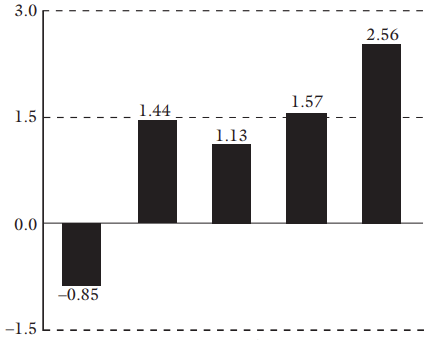
\includegraphics[scale=.5]{codigoFuente/tareas/pensamiento/img/1pensamiento.png}\\
	Quantiles EFI\\
	\small{Fuente: Gwartney y Lawson 2002,20}
    \end{center}

    Berggren (1999) encuentra que cuanto más aumentaba la libertad económica en un país entre 1975 y 1985, mayor era el grado de igualdad de ingresos de ese país alrededor de 1985. En particular, este resultado es válido para los países en desarrollo y para el momento en que se produjeron los cambios de política. liberalizó el comercio y desreguló el sistema financiero. La igualdad se mide como coeficientes de Gini y como comparaciones entre la participación en el ingreso o el consumo de personas con ingresos bajos y altos. Al mismo tiempo, el nivel de libertad económica en 1985 parece tener una relación negativa con la igualdad de ingresos, lo que probablemente sea un efecto de la redistribución reducida. Grubel (1998) da la vuelta al problema y estudia cómo la igualdad de ingresos afecta el PIB per cápita, el crecimiento económico y la libertad económica en diecisiete países con un PIB per cápita superior a 17.000 dólares. Los resultados sugieren que una mayor igualdad de ingresos está relacionada con un menor PIB per cápita, menor crecimiento y menor libertad económica. Scully (2002) estima un modelo estructural y modelos de forma reducida y muestra que la libertad económica es beneficiosa tanto para el crecimiento económico como para la igualdad porque tiene un efecto negativo significativo en los coeficientes de Gini. Además, una mayor igualdad reduce el crecimiento, pero solo en una pequeña cantidad.

    \section*{La libertad económica en contexto}
    Analizaremos la relación entre la libertad económica y otras variables tales como el PIB per cápita, el capital humano, el índice de desarrollo humano, el índice de desempeño ambiental, indice de Gini y el desempleo total.\\
    Para ello elaboramos y mostramos un gráfico multiple extraída de las distintas fuentes de datos para el año 2017 el cual se detalla a continuación. 


    \begin{center}
	Figura 3: Libertad económica en contexto.\\
	2017\\
	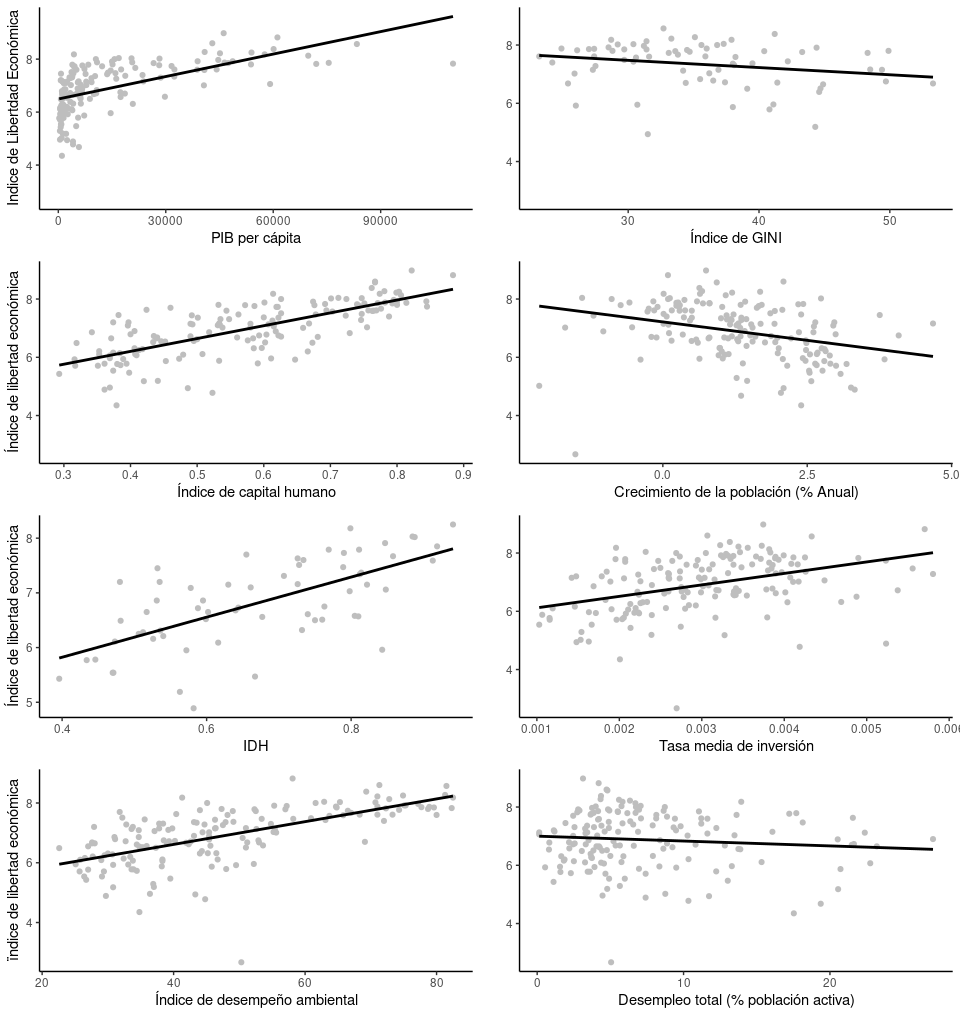
\includegraphics[scale=.65]{codigoFuente/tareas/pensamiento/img/multiplot.png}

	\small{Fuente: Banco Mundial y Universidad de Yale.}
    \end{center}

	\textbf{Relación con el PIB per cápita.}
	Como vimos en el anterior apartado la relación que existe entre la libertad económica y el PIB per cápita esta directamente o positivamente relacionado. Esto lo confirma la primera relación de la izquierda del gráfico 3. Donde a mayor puntuación en el índice se tendrá un PIB per cápita superior, es otras palabras a mayor PIB per cápita cualquier país recibirá una mejor puntación en el ranking. Esto se ve más clara si trazamos una linea de tendencia.\\\\

	\textbf{Relación con el capital humano.}
	Lo propio pasa cuando relacionamos la libertad económica y el capital humano. Como bien sabemos el capital humano es la parte más importante de cualquier organización el cual hace referencia a la productividad de los trabajadores que depende de su experiencia laboral y de su formación. Dicho un país goza de mayor libertad económica si la productividad de los trabajadores es mayor y mejor.\\\\

	\textbf{Relación con el índice de desarrollo humano.}
	A diferencia del capital humano en si, el índice de desarrollo humano se enfoca en tratar de promocionar el desarrollo potencial de las personas, el aumento de sus posibilidades, y el disfrute de la libertad para vivir la vida que valoran. Sabiendo este último y mostrado claramente en la parte inferior izquierda de la figura 3, vemos claramente una pendiente cerca de 1, el cual nos confirma que la libertad económica está positivamente correlacionada con la libertad para vivir, es decir, mayor IDH sugiere mayor libertad económica. \\\\


	\textbf{Relación con el índice de desempeño ambiental.}
	El Índice de Desempeño Ambiental (EPI por sus siglas en inglés: Environmental Performance Index), clasifica los países a partir de su desempeño en el logro de dos objetivos ambientales prioritarios: la salud ambiental que mide la protección de la salud humana ante el impacto de los daños ambientales; y la vitalidad de los ecosistemas que mide la protección a los ecosistemas y la administración de recursos. Este método para cuantificar y clasificar numéricamente el desempeño ambiental de las políticas de un país, esta claramente relaciono con la libertad económica, así se ve en el gráfico 3 en la parte superior derecha. A mejor puntación en el desempeño ambiental de un país, más libertad económica del mismo. A primera vista podría parecer ilógico esta afirmación pero la explicación partiría por el hecho de que a mayor libertad económica mayor políticas ambientales en un país.\\\\
	    
	\textbf{Relación con la Desigualdad y la distribución de la riqueza.}
	Para medir la desigualdad entre los habitantes de una población hacemos uso de la herramienta denominada indice de Gini. Este representa la desigualdad máxima que la cuantificamos con el número 1 o el 100, en cuyo caso uno solo de los habitantes recibiría el total de los ingresos por salarios. Por otro lado el 0, significa la igualdad total de los ingresos salariales de todos los habitantes. En este caso y según la gráfica 3 vemos que el índice de Gini esta negativamente relacionada con la libertad económica, en otras palabras podemos decir que mientras más desigualdad se tiene en un país más libertad económica existe.\\\\

	\textbf{Relación con el crecimiento de la población.}
	El crecimiento de una población se refiere, simplemente, al aumento, disminución o estabilidad en el número de sus integrantes en cada país, que ocurre en un período de tiempo determinado. Por lo que  vemos que a medida que el porcentaje de población anual aumenta entonces disminuye la libertad económica, por lo que nos muestra una pendiente ligeramente negativa.\\\\
    

	\textbf{Relación con la tasa media de inversión.}
	La tasa media de inversión prácticamente mide en cuanto ha crecido una inversión en un período determinado de tiempo. En este caso para el periodo de 2017 tenemos una relación positiva con respecto a la libertad económica, por lo que a medida que crece la tasa media de inversión también crecerá la libertad económica.\\\\

	\textbf{Relación con el desempleo.}
	El desempleo total de la población activa juega un rol interesante a la hora de relacionarse con la libertad económica de un país.\\
	Revisando la gráfica 3 en la parte inferior derecha, vemos que se tiene una ligera inclinación negativa entre el desempleo de un país y la libertad económica. Nos menciona que a mayor desempleo menor libertad económica y lo contrario a menor desempleo mayor libertad económica.  


\section*{La libertad económica y el crecimiento económico}
Una primera hipótesis propuesta por historiadores económicos como Aleksander Gerschenkron (1952) y MOses Abramovitz (1986) fue, que al menos en ciertas circunstancias, los países atrasados tenderían a crecer con más rapidez que los países ricos, este fenómeno se conoce como convergencia. A esto y con alguna investigación empírica llegamos a la conclusión de que algunos grupos de países si cumplen con la hipótesis dada y no así todo el conjunto de países del mundo. La pregunta es ¿Por qué? Para ello nos basamos en el modelo negoclásico.\\
Observemos la ecuación diferencial clave del modelo de crecimiento neoclásico,
$$\tilde{k}=s_K \tilde{y}-(n+g+d)\tilde{k}$$
Esta ecuación se puede escribir de nuevo como,
$$\dfrac{\tilde{k}}{\tilde{k}}=s_K \dfrac{\tilde{y}}{\tilde{k}}-(n+g+d)$$
Dónde podemos deducir que el producto promedio del capital disminuye según aumenta k debido a la acumulación de los rendimientos decrecientes de capital en el modelo neoclásico. Luego sabemos que la tasa de crecimiento de la tecnología es constante por lo que cualquier cambio de las tasas de crecimiento de $k$ e $y$ se debe atribuir a cambios en las tasas de crecimiento del capital por trabajador y de la producción por trabajador. Asi sacamos dos supuestos:
\begin{enumerate}
    \item Entre países que tienen el mismo estado estacionario, debe cumplirse la hipótesis de la convergencia: los países pobres deben crecer con mayor rapidez, en promedio, que los ricos.
    \item Principio de la dinámica de transición. Cuanto más se encuentre una economía por debajo de su estado estacionario con mayor rapidez deberá crecer y cuanto más por encima esté con mayor lentitud deberá crecer.
\end{enumerate}
Finalmente, la teoría de convergencia condicional se puede contrastar regresando la tasa de crecimiento del PIB pc, contra el logaritmo del PIB inicial y condicionando la regresión por las variables determinantes del estado estacionario,

$$\dfrac{1}{T}\ln\dfrac{Y_t}{Y_0}=B_0+B_1\ln Y_0 + B_2 X_2 + B_3 X_3 + \ldots + B_i X_i$$

Ya representados la tasa de crecimiento y el logaritmo de PIB per cápita inicial condicionado por las diferentes variables que determinan el PIB per cápita en el estado estacionario destacando que dentro de estas variables se encuentra la libertad económica y las diferentes variables explicativas del Instituto Fraser, además de otras variables que determinan el desempeño económico de un país a largo plazo, podremos realizar las distintas regresiones de convergencia.\\\\
Para tal efecto tendremos en cuenta la muestra de 112 países y algunos periodos de tiempo como los periodos de 1990-2017, 1990-2000, 2001-2007, 1990-2007 y 2008-2017. \\\\
La variable dependiente estará dada por:

\begin{center}
$PIBpc = \dfrac{1}{T}\ln\dfrac{Y_t}{Y_0}=y$ = tasa de crecimiento del PIB per cápita.

\end{center}

Las variables explicativas estarán dadas por: 

\begin{center}
\begin{tabular}{rcl}
    $lny_0$&=&Logaritmo del PIB per cápita inicial\\
    $ile_i$&=&Indice de libertad económica para el año final.\\
    $ile_0$&=&Índice de libertad económica inicial.\\
    $ tc_i$&=&Tasa de cambio del índice de libertad económica en el año final.\\
    $ich_i$&=&Índice de capital humano por trabajador en el año final.\\
    $tmi$&=&Tasa media de inversión de cada país durante el periodo de análisis.\\
    $n=tpob$&=&Tasa anual media de crecimiento de la población durante el periodo de análisis.\\
    $a1$&=&Área 1. Tamaño de gobierno.\\
    $a2$&=&Área 2. Sistema legal y derechos de propiedad.\\
    $a3$&=&Área 3. Moneada sólida.\\
    $a4$&=&Área 4. Libertad para comerciar internacionalmente.\\
    $a5$&=&Área 5. Regulación.\\
    $va$&=&Índice de calidad de gobernanza voice and Accountability.\\
    $PS=sav$&=&Índice de calidad de gobernanza Political Stability and Absence of Violence.\\\\
\end{tabular}
\end{center}

\subsection*{Regresiones de convergencia}
Para estas regresiones de convergencia analizaremos varios modelos con distintas variables explicativas.\\
\begin{enumerate}[\bfseries 1.]
   \item Primeramente utilizaremos las variables: valor del índice de libertad económica en el año inicial y el año final, donde introduciremos y sacaremos ambos de la regresión para ver cual es el que ayuda a explicar la tasa de crecimiento.
	$$\begin{array}{rcl}
	    y&=&\beta_0 + \beta_1\cdot lny_0 + \beta_2\cdot ile_i + \beta_3\cdot ile_0 + \beta_4\cdot tc_i + \beta_5\cdot ich_i + \beta_6\cdot tmi + \beta_7\cdot tpob + \epsilon\\\\
	    y&=&\beta_0 + \beta_1\cdot lny_0 + \beta_4\cdot tc_i + \beta_5\cdot ich_i + \beta_6\cdot tmi + \beta_7\cdot tpob + \epsilon\\\\
	\end{array}$$

    \item Probar introduciendo y sacando la tasa de cambio de índice de libertad económica para el año final con el objetivo de ver su poder explicativo.

	$$\begin{array}{rcl}
	    y&=&\beta_0 + \beta_1\cdot lny_0 + \beta_2\cdot ile_i + \beta_3\cdot ile_0 + \beta_4\cdot tc_i +\beta_5\cdot ich_i + \beta_6\cdot tmi + \beta_7\cdot tpob + \epsilon$$\\\\
	    y&=&\beta_0 + \beta_1\cdot lny_0 + \beta_2\cdot ile_i + \beta_3\cdot ile_0 + \beta_5\cdot ich_i + \beta_6\cdot tmi + \beta_7\cdot tpob + \epsilon$$\\\\
	\end{array}$$

    \item Probaremos  introduciendo diferentes componentes del índice de libertad económica para ver su capacidad explicativa de igual modo que hemos hecho con el índice agregado.

	$$\begin{array}{rcl}
	    y&=&\beta_0 + \beta_1\cdot lny_0 + \beta_5\cdot ich_i + \beta_6\cdot tmi + \beta_7\cdot tpob + \beta_{a1}\cdot a1 + \beta_{a2}\cdot a2  + \beta_{a3}\cdot a3 + \beta_{a4}\cdot a4 + \beta_{a5}\cdot a5 + \epsilon\\\\
	    y&=&\beta_0 + \beta_1\cdot lny_0 + \beta_5\cdot ich_i + \beta_6\cdot tmi + \beta_7\cdot tpob + \beta_{a1}\cdot a1 + \epsilon\\\\
	    y&=&\beta_0 + \beta_1\cdot lny_0 + \beta_5\cdot ich_i + \beta_6\cdot tmi + \beta_7\cdot tpob + \beta_{a2}\cdot a2 + \epsilon\\\\
	    y&=&\beta_0 + \beta_1\cdot lny_0 + \beta_5\cdot ich_i + \beta_6\cdot tmi + \beta_7\cdot tpob  + \beta_{a3}\cdot a3 + \epsilon\\\\
	    y&=&\beta_0 + \beta_1\cdot lny_0 + \beta_5\cdot ich_i + \beta_6\cdot tmi + \beta_7\cdot tpob + \beta_{a4}\cdot a4 + \epsilon\\\\
	    y&=&\beta_0 + \beta_1\cdot lny_0 + \beta_5\cdot ich_i + \beta_6\cdot tmi + \beta_7\cdot tpob + \beta_{a5}\cdot a5 + \epsilon\\\\
	\end{array}$$

    \item Por último Introduciremos como variables explicativas los índices de calidad de gobernanza Voice and Accountability y Political Stability and Absence of Violence elaborados por el Banco Mundial. Tomaremos el valor del último año del periodo de análisis.
	$$\begin{array}{rcl}
	    y&=&\beta_0 + \beta_1\cdot lny_0 + \beta_2\cdot ile_i + \beta_3\cdot ile_0 + \beta_4\cdot tc_i + \beta_5\cdot ich_i + \beta_6\cdot tmi + \beta_7\cdot tpob + \beta_{g1}\cdot va + \beta_{g2}\cdot sav + \epsilon\\\\
	    y&=&\beta_0 + \beta_1\cdot lny_0 + \beta_2\cdot ile_i + \beta_3\cdot ile_0 + \beta_4\cdot tc_i + \beta_5\cdot ich_i + \beta_6\cdot tmi + \beta_7\cdot tpob + \beta_{g1}\cdot va + \epsilon\\\\
	    y&=&\beta_0 + \beta_1\cdot lny_0 + \beta_2\cdot ile_i + \beta_3\cdot ile_0 + \beta_4\cdot tc_i + \beta_5\cdot ich_i + \beta_6\cdot tmi + \beta_7\cdot tpob + \beta_{g2}\cdot sav + \epsilon\\\\
	\end{array}$$

\end{enumerate}

	    \subsubsection*{Periodo 1990-2017}

		Según el cuadro 1 (Apéndice), vemos que los índices de libertad económica para el año inicial y final, explican a la tasa de crecimiento del PIB per cápita, esto, porque estás son significativas al $1\%$. Por el contrario y curiosamente, cuando obviamos las mismas, observamos que las demás variables como ser la tasa de cambio del índice económico y tasa media de inversión tasa anual media de crecimiento de la población se vuelven significativas.\\
		Según el cuadro 2, el poder explicativo de la tasa de cambio del índice de libertad económica es indistinta. Es decir, sea o no se incluya esta variable el $R^2$ no variara, pero si lo hara el estadístico F, con un aumento si esta variable no se toma en cuenta.\\  
		Con respecto a los diferentes componentes del índice de libertad económica los que más podrían explicar a la tasa de crecimiento del Pib pc son el sistema legal y derecho de propiedad y libertad para comercializar internacionalmente, eso si con un $R^2$ muy bajo en todos los casos pero un estadístico F algo.\\
		Por último cuando introducimos los índices de calidad de gobernanza vemos que el que mejor explica es Estabilidad Política y Ausencia de Violencia. 

	    \subsubsection*{Periodo 1990-2000}

		Contrario al periodo 1990-2017 vemos que la única variable significativa para poder explicar la tasa de crecimiento del PIB pc es el índice de libertad económica para el año final (2000), pero con buenos resultados para las demás variables explicativas como ser el índice de capital humano, tasa media de inversión y la tasa anual media de crecimiento de la población.\\
		Un buen modelo para este periodo podría ser obviando la tasa de cambio del índice de libertad económica, pero inversamente proporcional para casi toda las variables explicativas.\\
		Con respecto a las diferentes componentes del índice de libertad económica vemos que ninguna de estas es significativa, pero cada modelo explica levemente mejor que las del periodo 1990-2017.\\
		De igual forma al anterior periodo, al introducir los índices de calidad de gobernanza la que mejor variable que explica a la tasa de crecimiento del PIB pc es la estabilidad política y ausencia de violencia en un país, pero con casi todas variables negativas.\\

	    \subsubsection*{Periodo 2001-2007}
		
		Para este periodo observamos que las variables de índice de libertad económica para el año inicial y final no son significativas por lo tanto no explican de buena manera a la tasa de crecimiento del PIB pc.(Cuadro 9)\\
		Con respecto a introducir la tasa de cambio del índice de libertad económica, podría tener un poder explicativo pero muy leve.\\
		Por otro lado cuando incluimos los diferentes componentes del índice de libertad económica vemos que el que mejor podría explicar a la variable independiente es el sistema legal y derecho de propiedad pero con un poder explicativo muy bajo.\\
		Luego, contrario a los periodos 1990-2017 y 1990-2000 la variable que mejor aporta a explicar al PIB al incluir los índices de calidad de gobernanza es Voice and Accountability, pero de manera negativa, y un $R^2$ bajo (cuadro 12).\\

	    \subsubsection*{Periodo 1990-2007}
	    
		Como en el periodo 1990-2017 vemos que al introducir las respectivas variables del índice de libertad económica para el año inicial y final podría ayudar a explicar a la tasa de crecimiento pero con una significancia del $10\%$ y un $R^2$ del 0.2 (cuadro 13). Cabe mencionar que la tasa de cambio del índice de libertad económica para este periodo no tiene alguna relevancia.\\
		Con respecto a los componentes del índice de libertad, como vimos a un principio, las variables que explican y son significativas son el sistema legal y la libertad para comercializar. No pasa lo mismo con los índices de calidad de gobernanza donde ninguna es apropiada para explicar a la tasa de crecimiento.


	    \subsubsection*{Periodo 2008-2017}

		Al agregar los índices de libertad económica observamos que no son significativas para el modelo, pero si lo es la tasa de cambio. Contrario a esto, cuando excluimos la tasa de cambio los índices de libertad económica se vuelve significativas al $1\%$ con un $R^2$ de $0.34$.\\
		Cuando probamos incluir las componentes del índice de libertad la única que parece significativa es la de libertad comercial pero con un bajo poder explicativo.\\
		Por último y con un grado muy aceptable de poder explicativo a los índices de calidad de gobernanza.



    \section*{Conclusiones}

    Al poder realizar las distintas regresiones de covergencia, podemos notar que a través del tiempo las distintas variables que explican ala tasa de crecimiento, entre las cuales se encuentra el índice de libertad económica, toman mas protagonismo, esto podría deberse a la mejora continua al adquirir los distintos datos.\\
    
    Luego, podemos concluir que las variables que hacen referencia al índice de libertad económica no son del todo significativas si usamos paralelamente en el modelo esto por motivos de significancia y correlación. Por lo que para obtener un modelo donde estas variables sean significativas, y estén correlacionadas tendremos que escoger un modelo el cual suprimiera una de estas dos mantuviera la tasa de cambio del índice.\\

    Por otro lado concluimos  que los componentes del índice de libertad económica no trabajan bien en si incluimos sólo un componente, ya que algunos no son significativos. Mientras que si serán significativos si las estudiamos en conjunto.\\


\let\cleardoublepage\clearpage

\begin{thebibliography}{10}

    \bibitem[1]{}BERGGREN, Niclas. The benefits of economic freedom: a survey. The independent review, 2003, vol. 8, no 2, p. 193-211.

    \bibitem[2]{}DE HAAN, Jakob; LUNDSTR÷M, Susanna; STURM, Jan-Egbert. Marketoriented institutions and policies and economic growth: A critical survey. Journal of Economic Surveys, 2006, vol. 20, no 2, p. 157-191.
    \bibitem[3]{}ECONOMIC FREEDOM OF THE WORLD Annual Report 2020 (puedes también mirar los de anteriores años) https://www.fraserinstitute.org/studies/economic-freedom-of-the-world-2020-
annual-report https://www.fraserinstitute.org/sites/default/Öles/economic-freedom-of-theworld-2020.pdf
    \bibitem[4]{}JONES, Ch. I. . Introducción al crecimiento económico. Prentice Hall. (Especialmente la sección 3.2, la TeorÌa de la convergencia condicional, y también el capítulo 7 dedicado al análisis de la importancia de las instituciones política y económicas para el Éxito a largo plazo de los países)
    \bibitem[5]{}BARRO, R. J. y SALA-I-MARTIN, X. (1995). Economic Growth. McGrawHill. (Especialmente sección 1.2.8, 1.2.11, Tema 11)
\bibitem[6]{}\url{https://github.com/soyfode/ciencias_sociales/tree/master/economia/master/r/pensamientoEconomico}

\end{thebibliography}


\begin{comment}

    \section*{Apéndice}

%-------------------------------------------------------------------
%-----------------------------1-------------------------------------
\begin{table}[!htbp] \centering 
    \tiny
  \caption{} 
  \label{} 
\begin{tabular}{@{\extracolsep{5pt}}lcc} 
\\[-1.8ex]\hline 
\hline \\[-1.8ex] 
 & \multicolumn{2}{c}{\textit{Dependent variable:}} \\ 
\cline{2-3} 
\\[-1.8ex] & \multicolumn{2}{c}{y} \\ 
\\[-1.8ex] & (1) &(2)\\ 
\hline \\[-1.8ex] 
 lny\_0 & 0.001 & $-$0.0003 \\ 
  & p = 0.543 & p = 0.811 \\ 
  & & \\ 
 ile\_i & 0.018$^{***}$ &  \\ 
  & p = 0.001 &  \\ 
  & & \\ 
 ile\_0 & $-$0.012$^{**}$ &  \\ 
  & p = 0.037 &  \\ 
  & & \\ 
 tc\_i & $-$0.017 & 0.028$^{***}$ \\ 
  & p = 0.398 & p = 0.00003 \\ 
  & & \\ 
 ich\_i & $-$0.007 & $-$0.003 \\ 
  & p = 0.142 & p = 0.533 \\ 
  & & \\ 
 tmi & 0.050 & 0.083$^{**}$ \\ 
  & p = 0.147 & p = 0.021 \\ 
  & & \\ 
 tpob & $-$0.240 & $-$0.399$^{*}$ \\ 
  & p = 0.249 & p = 0.066 \\ 
  & & \\ 
 Constant & $-$0.007 & $-$0.014 \\ 
  & p = 0.809 & p = 0.468 \\ 
  & & \\ 
\hline \\[-1.8ex] 
Observations & 112 & 112 \\ 
R$^{2}$ & 0.324 & 0.219 \\ 
Adjusted R$^{2}$ & 0.278 & 0.182 \\ 
Residual Std. Error & 0.019 (df = 104) & 0.020 (df = 106) \\ 
F Statistic & 7.119$^{***}$ (df = 7; 104) & 5.952$^{***}$ (df = 5; 106) \\ 
\hline 
\hline \\[-1.8ex] 
\textit{Note:}  & \multicolumn{2}{r}{$^{*}$p$<$0.1; $^{**}$p$<$0.05; $^{***}$p$<$0.01} \\ 
\end{tabular} 
\end{table} 


\begin{table}[!htbp] \centering 
    \tiny
  \caption{} 
  \label{} 
\begin{tabular}{@{\extracolsep{5pt}}lcc} 
\\[-1.8ex]\hline 
\hline \\[-1.8ex] 
 & \multicolumn{2}{c}{\textit{Dependent variable:}} \\ 
\cline{2-3} 
\\[-1.8ex] & \multicolumn{2}{c}{y} \\ 
\\[-1.8ex] & (1) & (2)\\ 
\hline \\[-1.8ex] 
 lny\_0 & 0.001 & 0.0005 \\ 
  & p = 0.543 & p = 0.663 \\ 
  & & \\ 
 ile\_i & 0.018$^{***}$ & 0.014$^{***}$ \\ 
  & p = 0.001 & p = 0.00000 \\ 
  & & \\ 
 ile\_0 & $-$0.012$^{**}$ & $-$0.008$^{***}$ \\ 
  & p = 0.037 & p = 0.00003 \\ 
  & & \\ 
 tc\_i & $-$0.017 &  \\ 
  & p = 0.398 &  \\ 
  & & \\ 
 ich\_i & $-$0.007 & $-$0.008 \\ 
  & p = 0.142 & p = 0.103 \\ 
  & & \\ 
 tmi & 0.050 & 0.051 \\ 
  & p = 0.147 & p = 0.140 \\ 
  & & \\ 
 tpob & $-$0.240 & $-$0.269 \\ 
  & p = 0.249 & p = 0.192 \\ 
  & & \\ 
 Constant & $-$0.007 & $-$0.025 \\ 
  & p = 0.809 & p = 0.187 \\ 
  & & \\ 
\hline \\[-1.8ex] 
Observations & 112 & 112 \\ 
R$^{2}$ & 0.324 & 0.319 \\ 
Adjusted R$^{2}$ & 0.278 & 0.280 \\ 
Residual Std. Error & 0.019 (df = 104) & 0.019 (df = 105) \\ 
F Statistic & 7.119$^{***}$ (df = 7; 104) & 8.207$^{***}$ (df = 6; 105) \\ 
\hline 
\hline \\[-1.8ex] 
\textit{Note:}  & \multicolumn{2}{r}{$^{*}$p$<$0.1; $^{**}$p$<$0.05; $^{***}$p$<$0.01} \\ 
\end{tabular} 
\end{table} 


\begin{table}[!htbp] \centering 
    \tiny
  \caption{} 
  \label{} 
\begin{tabular}{@{\extracolsep{5pt}}lcccccc} 
\\[-1.8ex]\hline 
\hline \\[-1.8ex] 
 & \multicolumn{6}{c}{\textit{Dependent variable:}} \\ 
\cline{2-7} 
\\[-1.8ex] & \multicolumn{6}{c}{y} \\ 
\\[-1.8ex] & (1) & (2) &  (3) & (4) & (5) & (6)\\ 
\hline \\[-1.8ex] 
 lny\_0 & 0.0005 & $-$0.001 & $-$0.001 & $-$0.001 & 0.0003 & $-$0.001 \\ 
  & p = 0.738 & p = 0.640 & p = 0.595 & p = 0.690 & p = 0.834 & p = 0.557 \\ 
  & & & & & & \\ 
 ich\_i & 0.006 & $-$0.005 & 0.003 & $-$0.006 & 0.001 & $-$0.004 \\ 
  & p = 0.335 & p = 0.317 & p = 0.579 & p = 0.234 & p = 0.837 & p = 0.395 \\ 
  & & & & & & \\ 
 tmi & 0.095$^{**}$ & 0.072$^{*}$ & 0.099$^{**}$ & 0.078$^{**}$ & 0.090$^{**}$ & 0.077$^{**}$ \\ 
  & p = 0.019 & p = 0.060 & p = 0.011 & p = 0.046 & p = 0.023 & p = 0.048 \\ 
  & & & & & & \\ 
 tpob & $-$0.624$^{**}$ & $-$0.505$^{**}$ & $-$0.740$^{***}$ & $-$0.570$^{**}$ & $-$0.367 & $-$0.513$^{**}$ \\ 
  & p = 0.034 & p = 0.029 & p = 0.002 & p = 0.015 & p = 0.136 & p = 0.035 \\ 
  & & & & & & \\ 
 a1 & $-$0.002 & $-$0.001 &  &  &  &  \\ 
  & p = 0.310 & p = 0.409 &  &  &  &  \\ 
  & & & & & & \\ 
 a2 & $-$0.005$^{*}$ &  & $-$0.005$^{***}$ &  &  &  \\ 
  & p = 0.052 &  & p = 0.008 &  &  &  \\ 
  & & & & & & \\ 
 a3 & 0.0004 &  &  & $-$0.001 &  &  \\ 
  & p = 0.720 &  &  & p = 0.478 &  &  \\ 
  & & & & & & \\ 
 a4 & $-$0.002 &  &  &  & $-$0.003$^{***}$ &  \\ 
  & p = 0.117 &  &  &  & p = 0.005 &  \\ 
  & & & & & & \\ 
 a5 & 0.003 &  &  &  &  & $-$0.001 \\ 
  & p = 0.273 &  &  &  &  & p = 0.370 \\ 
  & & & & & & \\ 
 Constant & 0.024 & 0.042$^{**}$ & 0.038$^{**}$ & 0.040$^{**}$ & 0.021 & 0.042$^{**}$ \\ 
  & p = 0.264 & p = 0.025 & p = 0.019 & p = 0.017 & p = 0.233 & p = 0.013 \\ 
  & & & & & & \\ 
\hline \\[-1.8ex] 
Observations & 106 & 111 & 112 & 112 & 107 & 112 \\ 
R$^{2}$ & 0.170 & 0.082 & 0.138 & 0.083 & 0.142 & 0.086 \\ 
Adjusted R$^{2}$ & 0.092 & 0.039 & 0.098 & 0.040 & 0.100 & 0.043 \\ 
Residual Std. Error & 0.021 (df = 96) & 0.022 (df = 105) & 0.021 (df = 106) & 0.022 (df = 106) & 0.021 (df = 101) & 0.022 (df = 106) \\ 
F Statistic & 2.187$^{**}$ (df = 9; 96) & 1.881 (df = 5; 105) & 3.408$^{***}$ (df = 5; 106) & 1.924$^{*}$ (df = 5; 106) & 3.353$^{***}$ (df = 5; 101) & 1.990$^{*}$ (df = 5; 106) \\ 
\hline 
\hline \\[-1.8ex] 
\textit{Note:}  & \multicolumn{6}{r}{$^{*}$p$<$0.1; $^{**}$p$<$0.05; $^{***}$p$<$0.01} \\ 
\end{tabular} 
\end{table}




\begin{table}[!htbp] \centering 
    \tiny
  \caption{} 
  \label{} 
\begin{tabular}{@{\extracolsep{5pt}}lccc} 
\\[-1.8ex]\hline 
\hline \\[-1.8ex] 
 & \multicolumn{3}{c}{\textit{Dependent variable:}} \\ 
\cline{2-4} 
\\[-1.8ex] & \multicolumn{3}{c}{y} \\ 
\\[-1.8ex] & (1)  & (2) & (3)\\ 
\hline \\[-1.8ex] 
 lny\_0 & $-$0.001 & 0.0005 & $-$0.001 \\ 
  & p = 0.524 & p = 0.683 & p = 0.505 \\ 
  & & & \\ 
 ile\_i & 0.021$^{***}$ & 0.021$^{***}$ & 0.020$^{***}$ \\ 
  & p = 0.0003 & p = 0.0003 & p = 0.0002 \\ 
  & & & \\ 
 ile\_0 & $-$0.010$^{*}$ & $-$0.012$^{**}$ & $-$0.010$^{*}$ \\ 
  & p = 0.093 & p = 0.040 & p = 0.095 \\ 
  & & & \\ 
 tc\_i & $-$0.014 & $-$0.020 & $-$0.012 \\ 
  & p = 0.504 & p = 0.326 & p = 0.534 \\ 
  & & & \\ 
 ich\_i & $-$0.003 & $-$0.006 & $-$0.003 \\ 
  & p = 0.493 & p = 0.222 & p = 0.477 \\ 
  & & & \\ 
 tmi & 0.070$^{*}$ & 0.044 & 0.073$^{**}$ \\ 
  & p = 0.053 & p = 0.202 & p = 0.037 \\ 
  & & & \\ 
 tpob & $-$0.417$^{*}$ & $-$0.351 & $-$0.395$^{*}$ \\ 
  & p = 0.060 & p = 0.116 & p = 0.063 \\ 
  & & & \\ 
 va & $-$0.001 & $-$0.005 &  \\ 
  & p = 0.706 & p = 0.167 &  \\ 
  & & & \\ 
 sav & $-$0.009$^{**}$ &  & $-$0.009$^{***}$ \\ 
  & p = 0.026 &  & p = 0.010 \\ 
  & & & \\ 
 Constant & $-$0.039 & $-$0.018 & $-$0.037 \\ 
  & p = 0.203 & p = 0.542 & p = 0.213 \\ 
  & & & \\ 
\hline \\[-1.8ex] 
Observations & 112 & 112 & 112 \\ 
R$^{2}$ & 0.368 & 0.336 & 0.367 \\ 
Adjusted R$^{2}$ & 0.313 & 0.285 & 0.318 \\ 
Residual Std. Error & 0.019 (df = 102) & 0.019 (df = 103) & 0.018 (df = 103) \\ 
F Statistic & 6.608$^{***}$ (df = 9; 102) & 6.529$^{***}$ (df = 8; 103) & 7.478$^{***}$ (df = 8; 103) \\ 
\hline 
\hline \\[-1.8ex] 
\textit{Note:}  & \multicolumn{3}{r}{$^{*}$p$<$0.1; $^{**}$p$<$0.05; $^{***}$p$<$0.01} \\ 
\end{tabular} 
\end{table}


%----------------------------------------------------------------------------------
%----------------------------------- 2 --------------------------------------------

\begin{table}[!htbp] \centering 
    \tiny
  \caption{} 
  \label{} 
\begin{tabular}{@{\extracolsep{5pt}}lcc} 
\\[-1.8ex]\hline 
\hline \\[-1.8ex] 
 & \multicolumn{2}{c}{\textit{Dependent variable:}} \\ 
\cline{2-3} 
\\[-1.8ex] & \multicolumn{2}{c}{y} \\ 
\\[-1.8ex] & (1) & (2)\\ 
\hline \\[-1.8ex] 
 lny\_0 & 0.0004 & $-$0.001 \\ 
  & p = 0.789 & p = 0.587 \\ 
  & & \\ 
 ile\_i & 0.027$^{***}$ &  \\ 
  & p = 0.008 &  \\ 
  & & \\ 
 ile\_0 & $-$0.016 &  \\ 
  & p = 0.135 &  \\ 
  & & \\ 
 tc\_i & $-$0.041 & 0.018 \\ 
  & p = 0.285 & p = 0.107 \\ 
  & & \\ 
 ich\_i & $-$0.013$^{**}$ & $-$0.001 \\ 
  & p = 0.047 & p = 0.919 \\ 
  & & \\ 
 tmi & 0.091$^{***}$ & 0.126$^{***}$ \\ 
  & p = 0.007 & p = 0.0003 \\ 
  & & \\ 
 tpob & $-$0.481$^{*}$ & $-$0.554$^{*}$ \\ 
  & p = 0.081 & p = 0.055 \\ 
  & & \\ 
 Constant & $-$0.006 & $-$0.010 \\ 
  & p = 0.901 & p = 0.703 \\ 
  & & \\ 
\hline \\[-1.8ex] 
Observations & 112 & 112 \\ 
R$^{2}$ & 0.328 & 0.202 \\ 
Adjusted R$^{2}$ & 0.282 & 0.164 \\ 
Residual Std. Error & 0.025 (df = 104) & 0.027 (df = 106) \\ 
F Statistic & 7.239$^{***}$ (df = 7; 104) & 5.358$^{***}$ (df = 5; 106) \\ 
\hline 
\hline \\[-1.8ex] 
\textit{Note:}  & \multicolumn{2}{r}{$^{*}$p$<$0.1; $^{**}$p$<$0.05; $^{***}$p$<$0.01} \\ 
\end{tabular} 
\end{table}


\begin{table}[!htbp] \centering 
    \tiny
  \caption{} 
  \label{} 
\begin{tabular}{@{\extracolsep{5pt}}lcc} 
\\[-1.8ex]\hline 
\hline \\[-1.8ex] 
 & \multicolumn{2}{c}{\textit{Dependent variable:}} \\ 
\cline{2-3} 
\\[-1.8ex] & \multicolumn{2}{c}{y} \\ 
\\[-1.8ex] & (1) & (2)\\ 
\hline \\[-1.8ex] 
 lny\_0 & 0.0004 & 0.0001 \\ 
  & p = 0.789 & p = 0.931 \\ 
  & & \\ 
 ile\_i & 0.027$^{***}$ & 0.017$^{***}$ \\ 
  & p = 0.008 & p = 0.00002 \\ 
  & & \\ 
 ile\_0 & $-$0.016 & $-$0.005$^{*}$ \\ 
  & p = 0.135 & p = 0.080 \\ 
  & & \\ 
 tc\_i & $-$0.041 &  \\ 
  & p = 0.285 &  \\ 
  & & \\ 
 ich\_i & $-$0.013$^{**}$ & $-$0.014$^{**}$ \\ 
  & p = 0.047 & p = 0.034 \\ 
  & & \\ 
 tmi & 0.091$^{***}$ & 0.089$^{***}$ \\ 
  & p = 0.007 & p = 0.008 \\ 
  & & \\ 
 tpob & $-$0.481$^{*}$ & $-$0.542$^{**}$ \\ 
  & p = 0.081 & p = 0.045 \\ 
  & & \\ 
 Constant & $-$0.006 & $-$0.047$^{**}$ \\ 
  & p = 0.901 & p = 0.046 \\ 
  & & \\ 
\hline \\[-1.8ex] 
Observations & 112 & 112 \\ 
R$^{2}$ & 0.328 & 0.320 \\ 
Adjusted R$^{2}$ & 0.282 & 0.281 \\ 
Residual Std. Error & 0.025 (df = 104) & 0.025 (df = 105) \\ 
F Statistic & 7.239$^{***}$ (df = 7; 104) & 8.241$^{***}$ (df = 6; 105) \\ 
\hline 
\hline \\[-1.8ex] 
\textit{Note:}  & \multicolumn{2}{r}{$^{*}$p$<$0.1; $^{**}$p$<$0.05; $^{***}$p$<$0.01} \\ 
\end{tabular} 
\end{table} 


\begin{table}[!htbp] \centering 
    \tiny
  \caption{} 
  \label{} 
\begin{tabular}{@{\extracolsep{5pt}}lcccccc} 
\\[-1.8ex]\hline 
\hline \\[-1.8ex] 
 & \multicolumn{6}{c}{\textit{Dependent variable:}} \\ 
\cline{2-7} 
\\[-1.8ex] & \multicolumn{6}{c}{y} \\ 
\\[-1.8ex] & (1) & (2) & (3) & (4) & (5) & (6)\\ 
\hline \\[-1.8ex] 
 lny\_0 & $-$0.0004 & $-$0.001 & $-$0.001 & $-$0.001 & $-$0.0002 & $-$0.001 \\ 
  & p = 0.832 & p = 0.458 & p = 0.523 & p = 0.456 & p = 0.912 & p = 0.615 \\ 
  & & & & & & \\ 
 ich\_i & 0.002 & $-$0.001 & $-$0.004 & $-$0.003 & 0.001 & $-$0.004 \\ 
  & p = 0.791 & p = 0.895 & p = 0.571 & p = 0.634 & p = 0.847 & p = 0.524 \\ 
  & & & & & & \\ 
 tmi & 0.117$^{***}$ & 0.122$^{***}$ & 0.114$^{***}$ & 0.114$^{***}$ & 0.120$^{***}$ & 0.114$^{***}$ \\ 
  & p = 0.002 & p = 0.0005 & p = 0.002 & p = 0.002 & p = 0.001 & p = 0.002 \\ 
  & & & & & & \\ 
 tpob & $-$0.650$^{*}$ & $-$0.608$^{**}$ & $-$0.561$^{*}$ & $-$0.628$^{**}$ & $-$0.679$^{**}$ & $-$0.693$^{**}$ \\ 
  & p = 0.059 & p = 0.038 & p = 0.063 & p = 0.031 & p = 0.022 & p = 0.023 \\ 
  & & & & & & \\ 
 a1 & 0.00001 & 0.002 &  &  &  &  \\ 
  & p = 0.997 & p = 0.334 &  &  &  &  \\ 
  & & & & & & \\ 
 a2 & $-$0.0002 &  & 0.001 &  &  &  \\ 
  & p = 0.943 &  & p = 0.583 &  &  &  \\ 
  & & & & & & \\ 
 a3 & 0.002 &  &  & 0.001 &  &  \\ 
  & p = 0.251 &  &  & p = 0.308 &  &  \\ 
  & & & & & & \\ 
 a4 & $-$0.002 &  &  &  & $-$0.001 &  \\ 
  & p = 0.398 &  &  &  & p = 0.464 &  \\ 
  & & & & & & \\ 
 a5 & $-$0.0003 &  &  &  &  & 0.002 \\ 
  & p = 0.933 &  &  &  &  & p = 0.316 \\ 
  & & & & & & \\ 
 Constant & 0.004 & 0.006 & 0.017 & 0.017 & 0.009 & 0.013 \\ 
  & p = 0.864 & p = 0.809 & p = 0.394 & p = 0.411 & p = 0.651 & p = 0.550 \\ 
  & & & & & & \\ 
\hline \\[-1.8ex] 
Observations & 106 & 111 & 112 & 112 & 107 & 112 \\ 
R$^{2}$ & 0.243 & 0.197 & 0.184 & 0.190 & 0.225 & 0.190 \\ 
Adjusted R$^{2}$ & 0.172 & 0.158 & 0.146 & 0.152 & 0.187 & 0.151 \\ 
Residual Std. Error & 0.027 (df = 96) & 0.027 (df = 105) & 0.027 (df = 106) & 0.027 (df = 106) & 0.026 (df = 101) & 0.027 (df = 106) \\ 
F Statistic & 3.425$^{***}$ (df = 9; 96) & 5.139$^{***}$ (df = 5; 105) & 4.783$^{***}$ (df = 5; 106) & 4.965$^{***}$ (df = 5; 106) & 5.866$^{***}$ (df = 5; 101) & 4.957$^{***}$ (df = 5; 106) \\ 
\hline 
\hline \\[-1.8ex] 
\textit{Note:}  & \multicolumn{6}{r}{$^{*}$p$<$0.1; $^{**}$p$<$0.05; $^{***}$p$<$0.01} \\ 
\end{tabular} 
\end{table}



\begin{table}[!htbp] \centering 
    \tiny
  \caption{} 
  \label{} 
\begin{tabular}{@{\extracolsep{5pt}}lccc} 
\\[-1.8ex]\hline 
\hline \\[-1.8ex] 
 & \multicolumn{3}{c}{\textit{Dependent variable:}} \\ 
\cline{2-4} 
\\[-1.8ex] & \multicolumn{3}{c}{y} \\ 
\\[-1.8ex] & (1) & (2) & (3)\\ 
\hline \\[-1.8ex] 
 lny\_0 & 0.001 & 0.0004 & 0.001 \\ 
  & p = 0.378 & p = 0.777 & p = 0.399 \\ 
  & & & \\ 
 ile\_i & 0.027$^{***}$ & 0.026$^{**}$ & 0.024$^{**}$ \\ 
  & p = 0.010 & p = 0.015 & p = 0.015 \\ 
  & & & \\ 
 ile\_0 & $-$0.020$^{*}$ & $-$0.016 & $-$0.018$^{*}$ \\ 
  & p = 0.064 & p = 0.155 & p = 0.089 \\ 
  & & & \\ 
 tc\_i & $-$0.050 & $-$0.039 & $-$0.041 \\ 
  & p = 0.200 & p = 0.330 & p = 0.276 \\ 
  & & & \\ 
 ich\_i & $-$0.014$^{**}$ & $-$0.014$^{*}$ & $-$0.016$^{**}$ \\ 
  & p = 0.040 & p = 0.052 & p = 0.016 \\ 
  & & & \\ 
 tmi & 0.082$^{**}$ & 0.091$^{***}$ & 0.084$^{***}$ \\ 
  & p = 0.012 & p = 0.007 & p = 0.010 \\ 
  & & & \\ 
 tpob & $-$0.434 & $-$0.466$^{*}$ & $-$0.392 \\ 
  & p = 0.117 & p = 0.100 & p = 0.150 \\ 
  & & & \\ 
 va & $-$0.005 & 0.001 &  \\ 
  & p = 0.373 & p = 0.799 &  \\ 
  & & & \\ 
 sav & 0.011$^{**}$ &  & 0.009$^{**}$ \\ 
  & p = 0.014 &  & p = 0.021 \\ 
  & & & \\ 
 Constant & 0.021 & $-$0.005 & 0.020 \\ 
  & p = 0.644 & p = 0.921 & p = 0.654 \\ 
  & & & \\ 
\hline \\[-1.8ex] 
Observations & 112 & 112 & 112 \\ 
R$^{2}$ & 0.367 & 0.328 & 0.362 \\ 
Adjusted R$^{2}$ & 0.311 & 0.276 & 0.312 \\ 
Residual Std. Error & 0.025 (df = 102) & 0.025 (df = 103) & 0.025 (df = 103) \\ 
F Statistic & 6.572$^{***}$ (df = 9; 102) & 6.286$^{***}$ (df = 8; 103) & 7.307$^{***}$ (df = 8; 103) \\ 
\hline 
\hline \\[-1.8ex] 
\textit{Note:}  & \multicolumn{3}{r}{$^{*}$p$<$0.1; $^{**}$p$<$0.05; $^{***}$p$<$0.01} \\ 
\end{tabular} 
\end{table}


%------------------------------------------------------------------------
%------------------------------------3-----------------------------------

\begin{table}[!htbp] \centering 
    \tiny
  \caption{} 
  \label{} 
\begin{tabular}{@{\extracolsep{5pt}}lcc} 
\\[-1.8ex]\hline 
\hline \\[-1.8ex] 
 & \multicolumn{2}{c}{\textit{Dependent variable:}} \\ 
\cline{2-3} 
\\[-1.8ex] & \multicolumn{2}{c}{y} \\ 
\\[-1.8ex] & (1) & (2)\\ 
\hline \\[-1.8ex] 
 lny\_0 & 0.001 & 0.001 \\ 
  & p = 0.830 & p = 0.640 \\ 
  & & \\ 
 ile\_i & $-$0.066 &  \\ 
  & p = 0.149 &  \\ 
  & & \\ 
 ile\_0 & 0.064 &  \\ 
  & p = 0.161 &  \\ 
  & & \\ 
 tc\_i & 0.447$^{*}$ & 0.100$^{**}$ \\ 
  & p = 0.074 & p = 0.034 \\ 
  & & \\ 
 ich\_i & 0.001 & $-$0.001 \\ 
  & p = 0.947 & p = 0.892 \\ 
  & & \\ 
 tmi & 0.038 & 0.013 \\ 
  & p = 0.563 & p = 0.836 \\ 
  & & \\ 
 tpob & $-$0.255 & $-$0.197 \\ 
  & p = 0.440 & p = 0.544 \\ 
  & & \\ 
 Constant & $-$0.409 & $-$0.070 \\ 
  & p = 0.106 & p = 0.239 \\ 
  & & \\ 
\hline \\[-1.8ex] 
Observations & 118 & 118 \\ 
R$^{2}$ & 0.063 & 0.044 \\ 
Adjusted R$^{2}$ & 0.003 & 0.002 \\ 
Residual Std. Error & 0.044 (df = 110) & 0.044 (df = 112) \\ 
F Statistic & 1.054 (df = 7; 110) & 1.038 (df = 5; 112) \\ 
\hline 
\hline \\[-1.8ex] 
\textit{Note:}  & \multicolumn{2}{r}{$^{*}$p$<$0.1; $^{**}$p$<$0.05; $^{***}$p$<$0.01} \\ 
\end{tabular} 
\end{table} 



\begin{table}[!htbp] \centering 
    \tiny
  \caption{} 
  \label{} 
\begin{tabular}{@{\extracolsep{5pt}}lcc} 
\\[-1.8ex]\hline 
\hline \\[-1.8ex] 
 & \multicolumn{2}{c}{\textit{Dependent variable:}} \\ 
\cline{2-3} 
\\[-1.8ex] & \multicolumn{2}{c}{y} \\ 
\\[-1.8ex] & (1) & (2)\\ 
\hline \\[-1.8ex] 
 lny\_0 & 0.001 & 0.001 \\ 
  & p = 0.830 & p = 0.633 \\ 
  & & \\ 
 ile\_i & $-$0.066 & 0.014 \\ 
  & p = 0.149 & p = 0.133 \\ 
  & & \\ 
 ile\_0 & 0.064 & $-$0.017$^{*}$ \\ 
  & p = 0.161 & p = 0.066 \\ 
  & & \\ 
 tc\_i & 0.447$^{*}$ &  \\ 
  & p = 0.074 &  \\ 
  & & \\ 
 ich\_i & 0.001 & 0.001 \\ 
  & p = 0.947 & p = 0.927 \\ 
  & & \\ 
 tmi & 0.038 & 0.012 \\ 
  & p = 0.563 & p = 0.857 \\ 
  & & \\ 
 tpob & $-$0.255 & $-$0.164 \\ 
  & p = 0.440 & p = 0.618 \\ 
  & & \\ 
 Constant & $-$0.409 & 0.040 \\ 
  & p = 0.106 & p = 0.291 \\ 
  & & \\ 
\hline \\[-1.8ex] 
Observations & 118 & 118 \\ 
R$^{2}$ & 0.063 & 0.035 \\ 
Adjusted R$^{2}$ & 0.003 & $-$0.017 \\ 
Residual Std. Error & 0.044 (df = 110) & 0.044 (df = 111) \\ 
F Statistic & 1.054 (df = 7; 110) & 0.670 (df = 6; 111) \\ 
\hline 
\hline \\[-1.8ex] 
\textit{Note:}  & \multicolumn{2}{r}{$^{*}$p$<$0.1; $^{**}$p$<$0.05; $^{***}$p$<$0.01} \\ 
\end{tabular} 
\end{table}


\begin{table}[!htbp] \centering 
    \tiny
  \caption{} 
  \label{} 
\begin{tabular}{@{\extracolsep{5pt}}lcccccc} 
\\[-1.8ex]\hline 
\hline \\[-1.8ex] 
 & \multicolumn{6}{c}{\textit{Dependent variable:}} \\ 
\cline{2-7} 
\\[-1.8ex] & \multicolumn{6}{c}{y} \\ 
\\[-1.8ex] & (1) & (2) & (3) & (4) & (5) & (6)\\ 
\hline \\[-1.8ex] 
 lny\_0 & 0.003 & 0.001 & 0.001 & 0.001 & 0.001 & 0.001 \\ 
  & p = 0.295 & p = 0.711 & p = 0.667 & p = 0.726 & p = 0.745 & p = 0.784 \\ 
  & & & & & & \\ 
 ich\_i & 0.004 & $-$0.003 & 0.012 & 0.001 & $-$0.002 & $-$0.0001 \\ 
  & p = 0.752 & p = 0.761 & p = 0.246 & p = 0.903 & p = 0.835 & p = 0.992 \\ 
  & & & & & & \\ 
 tmi & 0.021 & 0.002 & 0.039 & 0.010 & 0.002 & 0.007 \\ 
  & p = 0.741 & p = 0.978 & p = 0.542 & p = 0.877 & p = 0.972 & p = 0.911 \\ 
  & & & & & & \\ 
 tpob & $-$0.604$^{*}$ & $-$0.207 & $-$0.246 & $-$0.152 & $-$0.192 & $-$0.165 \\ 
  & p = 0.088 & p = 0.531 & p = 0.452 & p = 0.648 & p = 0.571 & p = 0.624 \\ 
  & & & & & & \\ 
 a1 & $-$0.007$^{*}$ & $-$0.004 &  &  &  &  \\ 
  & p = 0.056 & p = 0.336 &  &  &  &  \\ 
  & & & & & & \\ 
 a2 & $-$0.015$^{***}$ &  & $-$0.008$^{**}$ &  &  &  \\ 
  & p = 0.003 &  & p = 0.039 &  &  &  \\ 
  & & & & & & \\ 
 a3 & $-$0.005 &  &  & $-$0.002 &  &  \\ 
  & p = 0.186 &  &  & p = 0.490 &  &  \\ 
  & & & & & & \\ 
 a4 & 0.009$^{*}$ &  &  &  & 0.001 &  \\ 
  & p = 0.086 &  &  &  & p = 0.840 &  \\ 
  & & & & & & \\ 
 a5 & 0.009 &  &  &  &  & $-$0.001 \\ 
  & p = 0.139 &  &  &  &  & p = 0.840 \\ 
  & & & & & & \\ 
 Constant & 0.052 & 0.067 & 0.037 & 0.047 & 0.039 & 0.044 \\ 
  & p = 0.256 & p = 0.108 & p = 0.214 & p = 0.147 & p = 0.218 & p = 0.242 \\ 
  & & & & & & \\ 
\hline \\[-1.8ex] 
Observations & 118 & 118 & 118 & 118 & 118 & 118 \\ 
R$^{2}$ & 0.104 & 0.013 & 0.042 & 0.009 & 0.005 & 0.005 \\ 
Adjusted R$^{2}$ & 0.030 & $-$0.031 & $-$0.001 & $-$0.035 & $-$0.039 & $-$0.039 \\ 
Residual Std. Error & 0.043 (df = 108) & 0.045 (df = 112) & 0.044 (df = 112) & 0.045 (df = 112) & 0.045 (df = 112) & 0.045 (df = 112) \\ 
F Statistic & 1.397 (df = 9; 108) & 0.298 (df = 5; 112) & 0.988 (df = 5; 112) & 0.207 (df = 5; 112) & 0.118 (df = 5; 112) & 0.118 (df = 5; 112) \\ 
\hline 
\hline \\[-1.8ex] 
\textit{Note:}  & \multicolumn{6}{r}{$^{*}$p$<$0.1; $^{**}$p$<$0.05; $^{***}$p$<$0.01} \\ 
\end{tabular} 
\end{table}


\begin{table}[!htbp] \centering 
    \tiny
  \caption{} 
  \label{} 
\begin{tabular}{@{\extracolsep{5pt}}lccc} 
\\[-1.8ex]\hline 
\hline \\[-1.8ex] 
 & \multicolumn{3}{c}{\textit{Dependent variable:}} \\ 
\cline{2-4} 
\\[-1.8ex] & \multicolumn{3}{c}{y} \\ 
\\[-1.8ex] & (1) & (2) & (3)\\ 
\hline \\[-1.8ex] 
 lny\_0 & $-$0.0004 & $-$0.001 & $-$0.0004 \\ 
  & p = 0.870 & p = 0.774 & p = 0.875 \\ 
  & & & \\ 
 ile\_i & $-$0.075$^{*}$ & $-$0.073$^{*}$ & $-$0.059 \\ 
  & p = 0.083 & p = 0.089 & p = 0.195 \\ 
  & & & \\ 
 ile\_0 & 0.090$^{**}$ & 0.088$^{**}$ & 0.061 \\ 
  & p = 0.041 & p = 0.044 & p = 0.186 \\ 
  & & & \\ 
 tc\_i & 0.566$^{**}$ & 0.552$^{**}$ & 0.418$^{*}$ \\ 
  & p = 0.018 & p = 0.020 & p = 0.095 \\ 
  & & & \\ 
 ich\_i & 0.011 & 0.012 & 0.005 \\ 
  & p = 0.282 & p = 0.212 & p = 0.614 \\ 
  & & & \\ 
 tmi & 0.026 & 0.029 & 0.046 \\ 
  & p = 0.672 & p = 0.632 & p = 0.484 \\ 
  & & & \\ 
 tpob & $-$0.635$^{*}$ & $-$0.615$^{*}$ & $-$0.238 \\ 
  & p = 0.053 & p = 0.057 & p = 0.470 \\ 
  & & & \\ 
 va & $-$0.032$^{***}$ & $-$0.030$^{***}$ &  \\ 
  & p = 0.0002 & p = 0.0001 &  \\ 
  & & & \\ 
 sav & 0.003 &  & $-$0.007 \\ 
  & p = 0.699 &  & p = 0.245 \\ 
  & & & \\ 
 Constant & $-$0.640$^{***}$ & $-$0.629$^{**}$ & $-$0.402 \\ 
  & p = 0.010 & p = 0.011 & p = 0.112 \\ 
  & & & \\ 
\hline \\[-1.8ex] 
Observations & 118 & 118 & 118 \\ 
R$^{2}$ & 0.191 & 0.190 & 0.074 \\ 
Adjusted R$^{2}$ & 0.124 & 0.131 & 0.007 \\ 
Residual Std. Error & 0.041 (df = 108) & 0.041 (df = 109) & 0.044 (df = 109) \\ 
F Statistic & 2.836$^{***}$ (df = 9; 108) & 3.196$^{***}$ (df = 8; 109) & 1.097 (df = 8; 109) \\ 
\hline 
\hline \\[-1.8ex] 
\textit{Note:}  & \multicolumn{3}{r}{$^{*}$p$<$0.1; $^{**}$p$<$0.05; $^{***}$p$<$0.01} \\ 
\end{tabular} 
\end{table}


%--------------------------------------------------------------------------
%---------------------------------------4----------------------------------


\begin{table}[!htbp] \centering 
    \tiny
  \caption{} 
  \label{} 
\begin{tabular}{@{\extracolsep{5pt}}lcc} 
\\[-1.8ex]\hline 
\hline \\[-1.8ex] 
 & \multicolumn{2}{c}{\textit{Dependent variable:}} \\ 
\cline{2-3} 
\\[-1.8ex] & \multicolumn{2}{c}{y} \\ 
\\[-1.8ex] & (1) & (2)\\ 
\hline \\[-1.8ex] 
 lny\_0 & 0.0005 & $-$0.0003 \\ 
  & p = 0.741 & p = 0.834 \\ 
  & & \\ 
 ile\_i & 0.015$^{*}$ &  \\ 
  & p = 0.054 &  \\ 
  & & \\ 
 ile\_0 & $-$0.015$^{*}$ &  \\ 
  & p = 0.086 &  \\ 
  & & \\ 
 tc\_i & $-$0.032 & 0.020$^{**}$ \\ 
  & p = 0.297 & p = 0.013 \\ 
  & & \\ 
 ich\_i & $-$0.002 & $-$0.002 \\ 
  & p = 0.744 & p = 0.741 \\ 
  & & \\ 
 tmi & 0.103$^{***}$ & 0.110$^{***}$ \\ 
  & p = 0.006 & p = 0.003 \\ 
  & & \\ 
 tpob & $-$0.331 & $-$0.430$^{*}$ \\ 
  & p = 0.176 & p = 0.073 \\ 
  & & \\ 
 Constant & 0.031 & $-$0.008 \\ 
  & p = 0.412 & p = 0.708 \\ 
  & & \\ 
\hline \\[-1.8ex] 
Observations & 112 & 112 \\ 
R$^{2}$ & 0.203 & 0.173 \\ 
Adjusted R$^{2}$ & 0.149 & 0.134 \\ 
Residual Std. Error & 0.023 (df = 104) & 0.024 (df = 106) \\ 
F Statistic & 3.778$^{***}$ (df = 7; 104) & 4.446$^{***}$ (df = 5; 106) \\ 
\hline 
\hline \\[-1.8ex] 
\textit{Note:}  & \multicolumn{2}{r}{$^{*}$p$<$0.1; $^{**}$p$<$0.05; $^{***}$p$<$0.01} \\ 
\end{tabular} 
\end{table}



\begin{table}[!htbp] \centering 
    \tiny
  \caption{} 
  \label{} 
\begin{tabular}{@{\extracolsep{5pt}}lcc} 
\\[-1.8ex]\hline 
\hline \\[-1.8ex] 
 & \multicolumn{2}{c}{\textit{Dependent variable:}} \\ 
\cline{2-3} 
\\[-1.8ex] & \multicolumn{2}{c}{y} \\ 
\\[-1.8ex] & (1) & (2)\\ 
\hline \\[-1.8ex] 
 lny\_0 & 0.0005 & 0.0001 \\ 
  & p = 0.741 & p = 0.918 \\ 
  & & \\ 
 ile\_i & 0.015$^{*}$ & 0.008$^{**}$ \\ 
  & p = 0.054 & p = 0.022 \\ 
  & & \\ 
 ile\_0 & $-$0.015$^{*}$ & $-$0.006$^{***}$ \\ 
  & p = 0.086 & p = 0.009 \\ 
  & & \\ 
 tc\_i & $-$0.032 &  \\ 
  & p = 0.297 &  \\ 
  & & \\ 
 ich\_i & $-$0.002 & $-$0.003 \\ 
  & p = 0.744 & p = 0.612 \\ 
  & & \\ 
 tmi & 0.103$^{***}$ & 0.103$^{***}$ \\ 
  & p = 0.006 & p = 0.006 \\ 
  & & \\ 
 tpob & $-$0.331 & $-$0.383 \\ 
  & p = 0.176 & p = 0.110 \\ 
  & & \\ 
 Constant & 0.031 & $-$0.001 \\ 
  & p = 0.412 & p = 0.968 \\ 
  & & \\ 
\hline \\[-1.8ex] 
Observations & 112 & 112 \\ 
R$^{2}$ & 0.203 & 0.194 \\ 
Adjusted R$^{2}$ & 0.149 & 0.148 \\ 
Residual Std. Error & 0.023 (df = 104) & 0.023 (df = 105) \\ 
F Statistic & 3.778$^{***}$ (df = 7; 104) & 4.221$^{***}$ (df = 6; 105) \\ 
\hline 
\hline \\[-1.8ex] 
\textit{Note:}  & \multicolumn{2}{r}{$^{*}$p$<$0.1; $^{**}$p$<$0.05; $^{***}$p$<$0.01} \\ 
\end{tabular} 
\end{table}



\begin{table}[!htbp] \centering 
    \tiny
  \caption{} 
  \label{} 
\begin{tabular}{@{\extracolsep{5pt}}lcccccc} 
\\[-1.8ex]\hline 
\hline \\[-1.8ex] 
 & \multicolumn{6}{c}{\textit{Dependent variable:}} \\ 
\cline{2-7} 
\\[-1.8ex] & \multicolumn{6}{c}{y} \\ 
\\[-1.8ex] & (1) & (2) & (3) & (4) & (5) & (6)\\ 
\hline \\[-1.8ex] 
 lny\_0 & 0.0001 & $-$0.001 & $-$0.001 & $-$0.0004 & 0.0003 & $-$0.001 \\ 
  & p = 0.942 & p = 0.709 & p = 0.673 & p = 0.768 & p = 0.819 & p = 0.608 \\ 
  & & & & & & \\ 
 ich\_i & 0.008 & $-$0.002 & 0.004 & $-$0.003 & 0.005 & $-$0.001 \\ 
  & p = 0.230 & p = 0.641 & p = 0.549 & p = 0.577 & p = 0.436 & p = 0.873 \\ 
  & & & & & & \\ 
 tmi & 0.122$^{***}$ & 0.106$^{***}$ & 0.121$^{***}$ & 0.104$^{***}$ & 0.118$^{***}$ & 0.108$^{***}$ \\ 
  & p = 0.003 & p = 0.004 & p = 0.002 & p = 0.006 & p = 0.002 & p = 0.004 \\ 
  & & & & & & \\ 
 tpob & $-$0.391 & $-$0.450$^{*}$ & $-$0.631$^{**}$ & $-$0.499$^{**}$ & $-$0.324 & $-$0.421$^{*}$ \\ 
  & p = 0.200 & p = 0.065 & p = 0.013 & p = 0.043 & p = 0.208 & p = 0.098 \\ 
  & & & & & & \\ 
 a1 & $-$0.001 & $-$0.001 &  &  &  &  \\ 
  & p = 0.776 & p = 0.591 &  &  &  &  \\ 
  & & & & & & \\ 
 a2 & $-$0.002 &  & $-$0.004$^{*}$ &  &  &  \\ 
  & p = 0.398 &  & p = 0.076 &  &  &  \\ 
  & & & & & & \\ 
 a3 & 0.001 &  &  & $-$0.001 &  &  \\ 
  & p = 0.448 &  &  & p = 0.632 &  &  \\ 
  & & & & & & \\ 
 a4 & $-$0.003$^{*}$ &  &  &  & $-$0.004$^{***}$ &  \\ 
  & p = 0.086 &  &  &  & p = 0.009 &  \\ 
  & & & & & & \\ 
 a5 & $-$0.0005 &  &  &  &  & $-$0.002 \\ 
  & p = 0.853 &  &  &  &  & p = 0.237 \\ 
  & & & & & & \\ 
 Constant & 0.013 & 0.028 & 0.028 & 0.028 & 0.011 & 0.033$^{*}$ \\ 
  & p = 0.562 & p = 0.157 & p = 0.108 & p = 0.121 & p = 0.568 & p = 0.075 \\ 
  & & & & & & \\ 
\hline \\[-1.8ex] 
Observations & 106 & 111 & 112 & 112 & 107 & 112 \\ 
R$^{2}$ & 0.195 & 0.136 & 0.149 & 0.125 & 0.180 & 0.135 \\ 
Adjusted R$^{2}$ & 0.119 & 0.095 & 0.109 & 0.084 & 0.139 & 0.094 \\ 
Residual Std. Error & 0.024 (df = 96) & 0.024 (df = 105) & 0.024 (df = 106) & 0.024 (df = 106) & 0.024 (df = 101) & 0.024 (df = 106) \\ 
F Statistic & 2.579$^{**}$ (df = 9; 96) & 3.313$^{***}$ (df = 5; 105) & 3.726$^{***}$ (df = 5; 106) & 3.041$^{**}$ (df = 5; 106) & 4.431$^{***}$ (df = 5; 101) & 3.312$^{***}$ (df = 5; 106) \\ 
\hline 
\hline \\[-1.8ex] 
\textit{Note:}  & \multicolumn{6}{r}{$^{*}$p$<$0.1; $^{**}$p$<$0.05; $^{***}$p$<$0.01} \\ 
\end{tabular} 
\end{table}



\begin{table}[!htbp] \centering 
    \tiny
  \caption{} 
  \label{} 
\begin{tabular}{@{\extracolsep{5pt}}lccc} 
\\[-1.8ex]\hline 
\hline \\[-1.8ex] 
 & \multicolumn{3}{c}{\textit{Dependent variable:}} \\ 
\cline{2-4} 
\\[-1.8ex] & \multicolumn{3}{c}{y} \\ 
\\[-1.8ex] & (1) & (2) & (3)\\ 
\hline \\[-1.8ex] 
 lny\_0 & 0.001 & 0.0002 & 0.001 \\ 
  & p = 0.548 & p = 0.878 & p = 0.620 \\ 
  & & & \\ 
 ile\_i & 0.021$^{***}$ & 0.020$^{**}$ & 0.015$^{*}$ \\ 
  & p = 0.009 & p = 0.014 & p = 0.053 \\ 
  & & & \\ 
 ile\_0 & $-$0.017$^{**}$ & $-$0.015$^{*}$ & $-$0.016$^{*}$ \\ 
  & p = 0.044 & p = 0.076 & p = 0.075 \\ 
  & & & \\ 
 tc\_i & $-$0.045 & $-$0.038 & $-$0.034 \\ 
  & p = 0.142 & p = 0.211 & p = 0.270 \\ 
  & & & \\ 
 ich\_i & $-$0.001 & 0.0004 & $-$0.003 \\ 
  & p = 0.898 & p = 0.948 & p = 0.671 \\ 
  & & & \\ 
 tmi & 0.088$^{**}$ & 0.093$^{**}$ & 0.101$^{***}$ \\ 
  & p = 0.019 & p = 0.012 & p = 0.007 \\ 
  & & & \\ 
 tpob & $-$0.460$^{*}$ & $-$0.485$^{*}$ & $-$0.309 \\ 
  & p = 0.071 & p = 0.057 & p = 0.216 \\ 
  & & & \\ 
 va & $-$0.010$^{**}$ & $-$0.009$^{**}$ &  \\ 
  & p = 0.026 & p = 0.050 &  \\ 
  & & & \\ 
 sav & 0.005 &  & 0.002 \\ 
  & p = 0.228 &  & p = 0.621 \\ 
  & & & \\ 
 Constant & 0.019 & 0.008 & 0.038 \\ 
  & p = 0.635 & p = 0.843 & p = 0.351 \\ 
  & & & \\ 
\hline \\[-1.8ex] 
Observations & 112 & 112 & 112 \\ 
R$^{2}$ & 0.243 & 0.232 & 0.205 \\ 
Adjusted R$^{2}$ & 0.176 & 0.172 & 0.143 \\ 
Residual Std. Error & 0.023 (df = 102) & 0.023 (df = 103) & 0.023 (df = 103) \\ 
F Statistic & 3.639$^{***}$ (df = 9; 102) & 3.892$^{***}$ (df = 8; 103) & 3.313$^{***}$ (df = 8; 103) \\ 
\hline 
\hline \\[-1.8ex] 
\textit{Note:}  & \multicolumn{3}{r}{$^{*}$p$<$0.1; $^{**}$p$<$0.05; $^{***}$p$<$0.01} \\ 
\end{tabular} 
\end{table}

%-----------------------------------------------------------------------
%-------------------------------5---------------------------------------


\begin{table}[!htbp] \centering 
    \tiny
  \caption{} 
  \label{} 
\begin{tabular}{@{\extracolsep{5pt}}lcc} 
\\[-1.8ex]\hline 
\hline \\[-1.8ex] 
 & \multicolumn{2}{c}{\textit{Dependent variable:}} \\ 
\cline{2-3} 
\\[-1.8ex] & \multicolumn{2}{c}{y} \\ 
\\[-1.8ex] & (1) & (2)\\ 
\hline \\[-1.8ex] 
 lny\_0 & $-$0.0005 & $-$0.001 \\ 
  & p = 0.822 & p = 0.562 \\ 
  & & \\ 
 ile\_i & $-$0.019 &  \\ 
  & p = 0.549 &  \\ 
  & & \\ 
 ile\_0 & 0.042 &  \\ 
  & p = 0.198 &  \\ 
  & & \\ 
 tc\_i & 0.438$^{***}$ & 0.300$^{***}$ \\ 
  & p = 0.007 & p = 0.000 \\ 
  & & \\ 
 ich\_i & $-$0.022$^{***}$ & $-$0.002 \\ 
  & p = 0.006 & p = 0.758 \\ 
  & & \\ 
 tmi & $-$0.103$^{**}$ & $-$0.058 \\ 
  & p = 0.042 & p = 0.268 \\ 
  & & \\ 
 tpob & $-$0.192 & $-$0.161 \\ 
  & p = 0.578 & p = 0.665 \\ 
  & & \\ 
 Constant & $-$0.490$^{***}$ & $-$0.252$^{***}$ \\ 
  & p = 0.004 & p = 0.00002 \\ 
  & & \\ 
\hline \\[-1.8ex] 
Observations & 131 & 131 \\ 
R$^{2}$ & 0.381 & 0.274 \\ 
Adjusted R$^{2}$ & 0.345 & 0.245 \\ 
Residual Std. Error & 0.039 (df = 123) & 0.041 (df = 125) \\ 
F Statistic & 10.802$^{***}$ (df = 7; 123) & 9.437$^{***}$ (df = 5; 125) \\ 
\hline 
\hline \\[-1.8ex] 
\textit{Note:}  & \multicolumn{2}{r}{$^{*}$p$<$0.1; $^{**}$p$<$0.05; $^{***}$p$<$0.01} \\ 
\end{tabular} 
\end{table}



\begin{table}[!htbp] \centering 
    \tiny
  \caption{} 
  \label{} 
\begin{tabular}{@{\extracolsep{5pt}}lcc} 
\\[-1.8ex]\hline 
\hline \\[-1.8ex] 
 & \multicolumn{2}{c}{\textit{Dependent variable:}} \\ 
\cline{2-3} 
\\[-1.8ex] & \multicolumn{2}{c}{y} \\ 
\\[-1.8ex] & (1) & (2)\\ 
\hline \\[-1.8ex] 
 lny\_0 & $-$0.0005 & $-$0.0004 \\ 
  & p = 0.822 & p = 0.868 \\ 
  & & \\ 
 ile\_i & $-$0.019 & 0.066$^{***}$ \\ 
  & p = 0.549 & p = 0.000 \\ 
  & & \\ 
 ile\_0 & 0.042 & $-$0.044$^{***}$ \\ 
  & p = 0.198 & p = 0.00001 \\ 
  & & \\ 
 tc\_i & 0.438$^{***}$ &  \\ 
  & p = 0.007 &  \\ 
  & & \\ 
 ich\_i & $-$0.022$^{***}$ & $-$0.024$^{***}$ \\ 
  & p = 0.006 & p = 0.004 \\ 
  & & \\ 
 tmi & $-$0.103$^{**}$ & $-$0.106$^{**}$ \\ 
  & p = 0.042 & p = 0.042 \\ 
  & & \\ 
 tpob & $-$0.192 & $-$0.174 \\ 
  & p = 0.578 & p = 0.625 \\ 
  & & \\ 
 Constant & $-$0.490$^{***}$ & $-$0.040 \\ 
  & p = 0.004 & p = 0.262 \\ 
  & & \\ 
\hline \\[-1.8ex] 
Observations & 131 & 131 \\ 
R$^{2}$ & 0.381 & 0.342 \\ 
Adjusted R$^{2}$ & 0.345 & 0.310 \\ 
Residual Std. Error & 0.039 (df = 123) & 0.040 (df = 124) \\ 
F Statistic & 10.802$^{***}$ (df = 7; 123) & 10.719$^{***}$ (df = 6; 124) \\ 
\hline 
\hline \\[-1.8ex] 
\textit{Note:}  & \multicolumn{2}{r}{$^{*}$p$<$0.1; $^{**}$p$<$0.05; $^{***}$p$<$0.01} \\ 
\end{tabular} 
\end{table}




\begin{table}[!htbp] \centering 
    \tiny
  \caption{} 
  \label{} 
  \begin{turn}{0}
\begin{tabular}{@{\extracolsep{5pt}}lcccccc} 
\\[-1.8ex]\hline 
\hline \\[-1.8ex] 
 & \multicolumn{6}{c}{\textit{Dependent variable:}} \\ 
\cline{2-7} 
\\[-1.8ex] & \multicolumn{6}{c}{y} \\ 
\\[-1.8ex] & (1) & (2) & (3) & (4) & (5) & (6)\\ 
\hline \\[-1.8ex] 
 lny\_0 & $-$0.001 & $-$0.001 & $-$0.002 & $-$0.002 & $-$0.001 & $-$0.002 \\ 
  & p = 0.689 & p = 0.710 & p = 0.444 & p = 0.446 & p = 0.564 & p = 0.537 \\ 
  & & & & & & \\ 
 ich\_i & $-$0.015 & $-$0.009 & $-$0.013 & $-$0.010 & $-$0.019$^{**}$ & $-$0.011 \\ 
  & p = 0.150 & p = 0.257 & p = 0.178 & p = 0.251 & p = 0.038 & p = 0.240 \\ 
  & & & & & & \\ 
 tmi & 0.027 & 0.055 & $-$0.020 & $-$0.006 & $-$0.022 & $-$0.004 \\ 
  & p = 0.679 & p = 0.359 & p = 0.752 & p = 0.922 & p = 0.713 & p = 0.948 \\ 
  & & & & & & \\ 
 tpob & $-$0.268 & $-$0.454 & $-$0.387 & $-$0.431 & $-$0.455 & $-$0.503 \\ 
  & p = 0.549 & p = 0.267 & p = 0.369 & p = 0.314 & p = 0.280 & p = 0.261 \\ 
  & & & & & & \\ 
 a1 & 0.012$^{***}$ & 0.013$^{***}$ &  &  &  &  \\ 
  & p = 0.003 & p = 0.001 &  &  &  &  \\ 
  & & & & & & \\ 
 a2 & 0.005 &  & 0.003 &  &  &  \\ 
  & p = 0.280 &  & p = 0.402 &  &  &  \\ 
  & & & & & & \\ 
 a3 & $-$0.006 &  &  & 0.002 &  &  \\ 
  & p = 0.241 &  &  & p = 0.647 &  &  \\ 
  & & & & & & \\ 
 a4 & 0.009 &  &  &  & 0.009$^{**}$ &  \\ 
  & p = 0.136 &  &  &  & p = 0.029 &  \\ 
  & & & & & & \\ 
 a5 & $-$0.006 &  &  &  &  & 0.003 \\ 
  & p = 0.342 &  &  &  &  & p = 0.596 \\ 
  & & & & & & \\ 
 Constant & $-$0.029 & $-$0.048 & 0.068$^{**}$ & 0.061$^{*}$ & 0.033 & 0.055 \\ 
  & p = 0.564 & p = 0.297 & p = 0.045 & p = 0.090 & p = 0.361 & p = 0.183 \\ 
  & & & & & & \\ 
\hline \\[-1.8ex] 
Observations & 131 & 131 & 131 & 131 & 131 & 131 \\ 
R$^{2}$ & 0.138 & 0.109 & 0.026 & 0.022 & 0.057 & 0.023 \\ 
Adjusted R$^{2}$ & 0.074 & 0.073 & $-$0.013 & $-$0.017 & 0.020 & $-$0.016 \\ 
Residual Std. Error & 0.046 (df = 121) & 0.046 (df = 125) & 0.048 (df = 125) & 0.048 (df = 125) & 0.047 (df = 125) & 0.048 (df = 125) \\ 
F Statistic & 2.153$^{**}$ (df = 9; 121) & 3.058$^{**}$ (df = 5; 125) & 0.669 (df = 5; 125) & 0.568 (df = 5; 125) & 1.524 (df = 5; 125) & 0.583 (df = 5; 125) \\ 
\hline 
\hline \\[-1.8ex] 
\textit{Note:}  & \multicolumn{6}{r}{$^{*}$p$<$0.1; $^{**}$p$<$0.05; $^{***}$p$<$0.01} \\ 
\end{tabular} 
\end{turn}
\end{table}



\begin{table}[!htbp] \centering 
    \tiny
  \caption{} 
  \label{} 
\begin{tabular}{@{\extracolsep{5pt}}lccc} 
\\[-1.8ex]\hline 
\hline \\[-1.8ex] 
 & \multicolumn{3}{c}{\textit{Dependent variable:}} \\ 
\cline{2-4} 
\\[-1.8ex] & \multicolumn{3}{c}{y} \\ 
\\[-1.8ex] & (1) & (2) & (3)\\ 
\hline \\[-1.8ex] 
 lny\_0 & $-$0.003 & $-$0.001 & $-$0.003 \\ 
  & p = 0.251 & p = 0.663 & p = 0.213 \\ 
  & & & \\ 
 ile\_i & $-$0.013 & $-$0.017 & $-$0.014 \\ 
  & p = 0.664 & p = 0.587 & p = 0.663 \\ 
  & & & \\ 
 ile\_0 & 0.045 & 0.046 & 0.043 \\ 
  & p = 0.153 & p = 0.151 & p = 0.172 \\ 
  & & & \\ 
 tc\_i & 0.436$^{***}$ & 0.442$^{***}$ & 0.433$^{***}$ \\ 
  & p = 0.006 & p = 0.006 & p = 0.006 \\ 
  & & & \\ 
 ich\_i & $-$0.014$^{*}$ & $-$0.020$^{**}$ & $-$0.014 \\ 
  & p = 0.098 & p = 0.012 & p = 0.108 \\ 
  & & & \\ 
 tmi & $-$0.048 & $-$0.095$^{*}$ & $-$0.040 \\ 
  & p = 0.384 & p = 0.057 & p = 0.462 \\ 
  & & & \\ 
 tpob & $-$0.306 & $-$0.333 & $-$0.237 \\ 
  & p = 0.377 & p = 0.340 & p = 0.485 \\ 
  & & & \\ 
 va & $-$0.006 & $-$0.012$^{**}$ &  \\ 
  & p = 0.314 & p = 0.047 &  \\ 
  & & & \\ 
 sav & $-$0.014$^{*}$ &  & $-$0.017$^{**}$ \\ 
  & p = 0.065 &  & p = 0.012 \\ 
  & & & \\ 
 Constant & $-$0.561$^{***}$ & $-$0.537$^{***}$ & $-$0.546$^{***}$ \\ 
  & p = 0.001 & p = 0.002 & p = 0.002 \\ 
  & & & \\ 
\hline \\[-1.8ex] 
Observations & 131 & 131 & 131 \\ 
R$^{2}$ & 0.417 & 0.401 & 0.412 \\ 
Adjusted R$^{2}$ & 0.374 & 0.361 & 0.374 \\ 
Residual Std. Error & 0.038 (df = 121) & 0.038 (df = 122) & 0.038 (df = 122) \\ 
F Statistic & 9.631$^{***}$ (df = 9; 121) & 10.195$^{***}$ (df = 8; 122) & 10.705$^{***}$ (df = 8; 122) \\ 
\hline 
\hline \\[-1.8ex] 
\textit{Note:}  & \multicolumn{3}{r}{$^{*}$p$<$0.1; $^{**}$p$<$0.05; $^{***}$p$<$0.01} \\ 
\end{tabular} 
\end{table} 
\end{comment}
